In this section we study the interaction of a so called "coronal hole" with an MHD wave. 
A coronal hole is a region in the coronal with musch lower pressure and density than the surrounding area.
In fuigure \autoref{fig:coronal-hole} you can see a series of plots of the pressure wave interacting with the coronal hole.

\begin{figure}[H]
	%\hspace{-1cm}
	\centering
	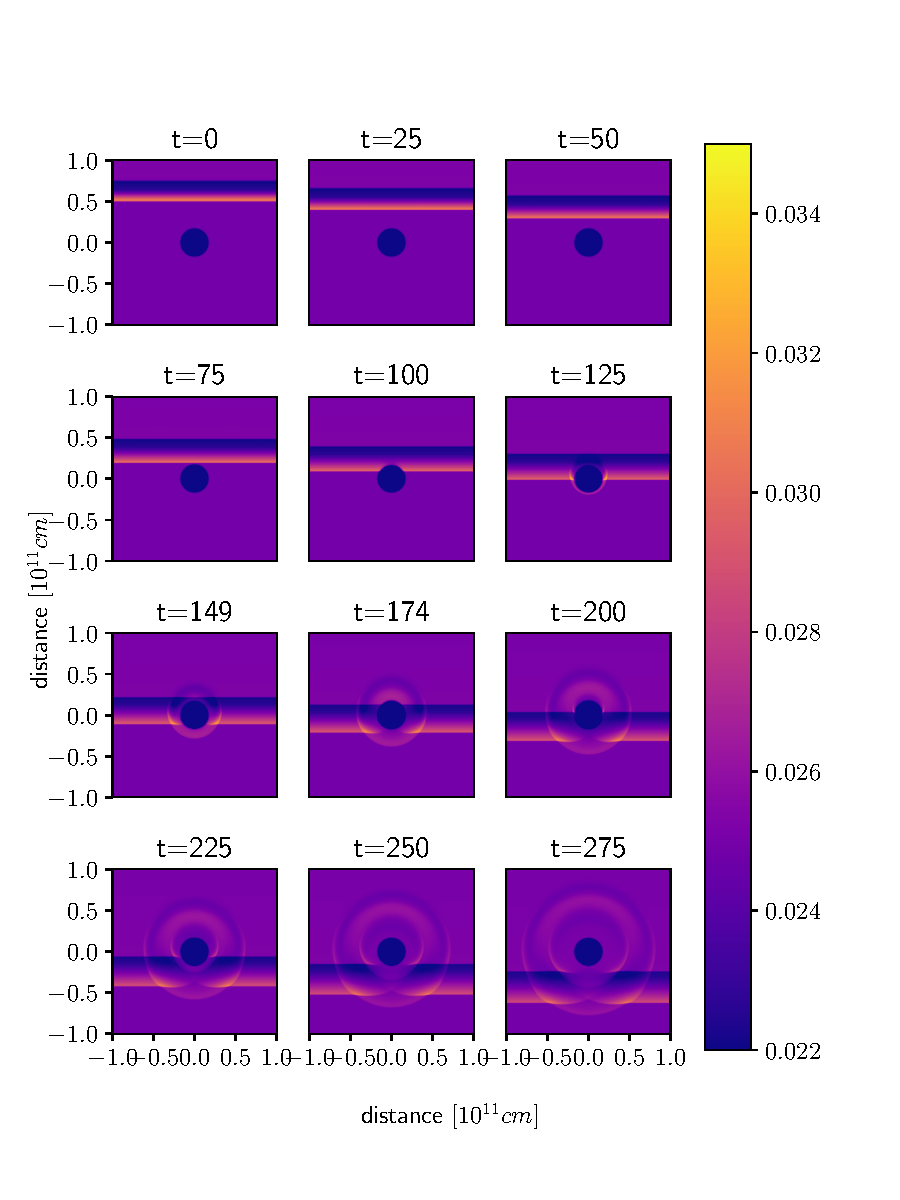
\includegraphics[width=\linewidth]{images/coronal-hole.pdf}
	\caption{Interaction of shock wave with coronal hole plotted at different times.}
	\label{fig:coronal-hole}
\end{figure}

The refraction and reflection of the wave around the coronal hole is clearly visible, the group speed inside the hole is slower than outside.

\todo[inline]{add plots wit initial conditions and form of wave driver}
\todo[inline]{add discussion of simulation results: refraction effects}
\todo[inline]{add short discussion of coronal plume}
